% Compile with pdflatex

\documentclass[a4paper,10pt]{report}

\usepackage[utf8]{inputenc}
\usepackage{pgfplots}
\usepackage{tikz}

% \pgfplotsset{width=7cm,compat=1.8}

% Title Page
\title{The Logarithmic Filter}
\author{José M. González}


\begin{document}
\maketitle

\begin{abstract}
This document explains the equations for building a logarithmic filter.
\end{abstract}

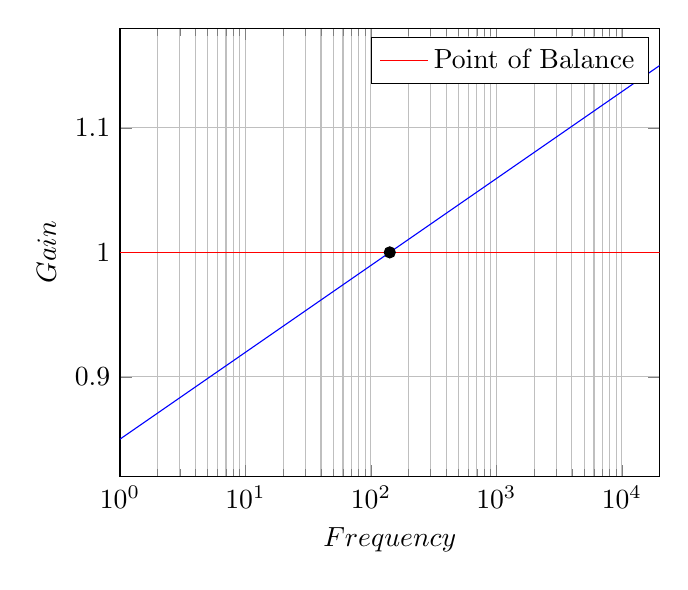
\begin{tikzpicture}
  \begin{semilogxaxis}[
    xmin=1, xmax=2e4, domain=1:20000,
    grid=both,
    xlabel=$Frequency$,
    ylabel=$Gain$
  ]

    \addplot[red] {1};
    \addlegendentry{Point of Balance} 

    \addplot[blue] {0.030292359 * ln(x) + 0.85 };
   
    \addplot[black, mark=*] 
            plot[errors bars/.cd]
            coordinates {(141.421356237,1)};
    
  
  \end{semilogxaxis}
\end{tikzpicture}

$Gain=1$ Point of Balance

$$G=m \log_s{f} - \log_s{B}$$

G: Gain \\
s: Scale \\
f: Frequency \\
B: Point of Balance \\
m: slope


$$G = m \frac{\ln{f}}{\ln{s}} - \frac{\ln{B}}{\ln{s}} $$

If $G$ is defined as $1 \pm \delta $ we get, some useful equations.

\begin{eqnarray} 
  2 \delta & = & \frac{m}{\ln{s}} \ln { \frac{F_{MAX}}{ F_{MIN} } } \\
  m & = & \frac{- \delta}{1-\delta} = \frac{\delta}{\delta - 1} \\
  \ln{s} & = &\frac{m}{2 \delta} \ln{ \frac{F_{MAX}}{ F_{MIN} } }  \\
  \ln{s} & = & \frac{1}{2 (\delta - 1)} \ln{ \frac{F_{MAX}}{ F_{MIN} } } \\
  \ln{B} & = & \frac{\ln{s}}{m-1} \\
  \ln{B} & = & \frac{1}{2} \ln { \frac{F_{MAX}}{ F_{MIN} } }
\end{eqnarray}

A non logarithmic representation:


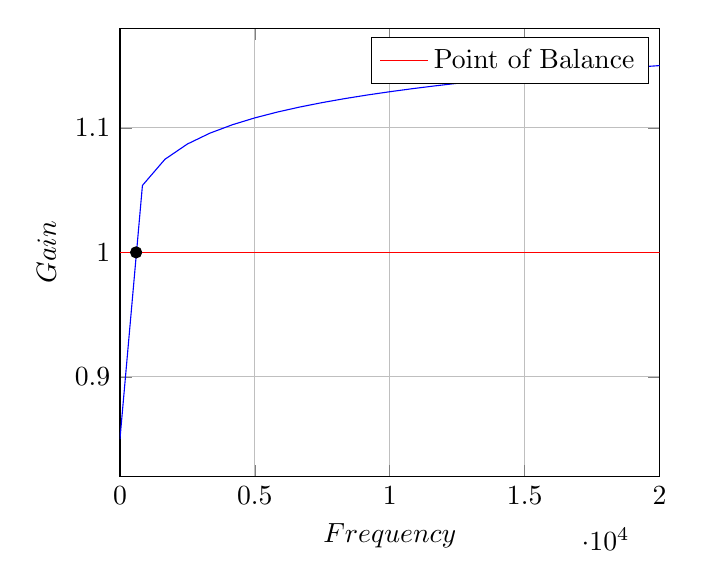
\begin{tikzpicture}
  \begin{axis}[
    xmin=1, xmax=2e4, domain=1:20000,
    grid=both,
    xlabel=$Frequency$,
    ylabel=$Gain$
  ]

    \addplot[red] {1};
    \addlegendentry{Point of Balance} 

    \addplot[blue] {0.030292359 * ln(x) + 0.85 };
   
    \addplot[black, mark=*] 
            plot[errors bars/.cd]
            coordinates {(600, 1)};
    
  \end{axis}
\end{tikzpicture}

\end{document}          

Transfer Function

Impulse response